\documentclass[10pt,conference,a4paper]{IEEEtran}
\usepackage[T1]{fontenc}
\usepackage{times}
\usepackage{helvet}
\usepackage{graphicx}
\usepackage{amsmath}
\usepackage{booktabs}
\usepackage{url}
\raggedbottom

% Required font spec (per supervisor): title 24pt Times, abstract 9pt bold-italic Times,
% body 10pt Times, headings 10pt bold Times, figure/table captions 8pt Helvetica/Arial,
% references 8pt Times. IEEEtran's default conference styling already gives a 24pt title,
% a 9pt bold-italic abstract, 10pt body, and 8pt Times references (\footnotesize inside
% \thebibliography) once Times is loaded above. Section headings default to small caps
% rather than bold in conference mode, and captions default to 8pt Times rather than
% Helvetica, so both are overridden explicitly below (no external caption package needed).
\makeatletter
\def\section{\@startsection{section}{1}{\z@}{1.5ex plus 1.5ex minus 0.5ex}%
{0.7ex plus 1ex minus 0ex}{\normalfont\normalsize\bfseries\centering}}%

\long\def\@makecaption#1#2{%
\ifx\@captype\@IEEEtablestring%
\footnotesize\sffamily\bgroup\par\centering\@IEEEtabletopskipstrut{\sffamily\footnotesize #1}\\{\sffamily\footnotesize #2}\par\addvspace{0.5\baselineskip}\egroup%
\@IEEEtablecaptionsepspace
\else
\@IEEEfigurecaptionsepspace
\setbox\@tempboxa\hbox{\sffamily\footnotesize {#1.}\nobreakspace\nobreakspace #2}%
\ifdim \wd\@tempboxa >\hsize%
\setbox\@tempboxa\hbox{\sffamily\footnotesize {#1.}\nobreakspace\nobreakspace}%
\parbox[t]{\hsize}{\sffamily\footnotesize\noindent\unhbox\@tempboxa#2}%
\else%
\ifCLASSOPTIONconference \hbox to\hsize{\sffamily\footnotesize\hfil\box\@tempboxa\hfil}%
\else \hbox to\hsize{\sffamily\footnotesize\box\@tempboxa\hfil}%
\fi\fi\fi}
\makeatother

\begin{document}
\pagestyle{plain}

\title{PAE-Weighted Graph Neural Networks for Missense Variant Pathogenicity Prediction}

\author{
\IEEEauthorblockN{Megha Kanojia}
\IEEEauthorblockA{School of Computing\\Dublin City University\\Dublin, Ireland\\megha.kanojia2@mail.dcu.ie}
\and
\IEEEauthorblockN{Aadesh Sunil Kshetre}
\IEEEauthorblockA{School of Computing\\Dublin City University\\Dublin, Ireland\\aadeshsunil.kshetre2@mail.dcu.ie}
}

\maketitle
\thispagestyle{plain}

\begin{abstract}
A missense variant is a single-letter DNA change that alters a protein and can cause disease. Of the more than four million such variants observed in the human genome, only about 2\% have a confirmed pathogenic or benign classification, and manual wet-lab validation is too costly and slow to close this gap at scale, making computational prediction necessary. Tools such as AlphaMissense already use AlphaFold2's predicted protein structures for this task. This paper tests a narrower question: does weighting each structural contact by AlphaFold2's confidence in that contact, given by its Predicted Aligned Error (PAE) score, improve pathogenicity prediction over treating every contact as equally reliable? We built a Graph Attention Network v2 (GATv2) combining protein contact graphs with ESM-2 sequence embeddings, trained on 49,303 high-confidence ClinVar missense variants across 6,597 proteins, and compared a PAE-weighted model against an unweighted ablation, GCN, GraphSAGE, XGBoost, and AlphaMissense. Two further, architecturally distinct PAE encodings were tested to rule out the specific transform as the cause of any null result. At the tuned stage used for the main comparison, none of the three encodings significantly improved on the unweighted ablation (bootstrap $p=0.073$-$0.698$, DeLong $p=0.067$-$0.901$); the one significant result among six comparisons pointed toward PAE-weighting hurting, not helping. A diagnostic traced this to AlphaFold's PAE values being heavily compressed for residue pairs close enough to pass the contact cutoff. GraphSAGE was the best-performing model built here (AUPRC 0.9148), and AlphaMissense remained significantly ahead of every model tested (AUPRC 0.9286, $p<0.001$). We report this as a rigorously tested negative result with a clear mechanistic explanation, not a failed experiment.
\end{abstract}
\begin{IEEEkeywords}
missense variants, pathogenicity prediction, graph neural network, graph attention network, AlphaFold, predicted aligned error, ClinVar, protein language model
\end{IEEEkeywords}

\section{Introduction}

DNA acts as the blueprint for the proteins that carry out almost every function in the human body. A \textit{missense variant} is a single-letter change in that blueprint that swaps one amino acid in a protein for another. Most of the time this substitution is harmless. Occasionally, though, it disrupts how the protein folds or functions, and disease follows \cite{zhang2012missense}. Telling the harmful (\textit{pathogenic}) substitutions apart from the harmless (\textit{benign}) ones is one of the central open problems in clinical genomics \cite{ciesielski2024context}. Of more than four million missense variants catalogued in humans, only around 2\% currently have a confirmed clinical classification \cite{cheng2023alphamissense}. The rest are labelled \textit{Variants of Uncertain Significance} (VUS), leaving patients and clinicians with no answer at all. Manually testing a single variant in a wet lab can cost thousands of dollars and take months \cite{santosgonzalez2024cost}. Hence, computational prediction is the best approach to analyze them efficiently.

Two pieces of technology make a new kind of computational predictor possible. The first is \textbf{AlphaFold2}, which predicts a protein's 3D shape directly from its sequence \cite{jumper2021alphafold}. For every pair of amino acids in that predicted structure, AlphaFold2 also reports a confidence score called \textit{Predicted Aligned Error} (PAE): an estimate, in \r{A}ngstr\"{o}ms, of how much the model trusts the relative position of that specific pair. A low PAE value indicates high confidence in the predicted relative position of that residue pair, while a high PAE value indicates greater positional uncertainty. The second technology is \textbf{ESM-2}, a large language model trained on protein sequences much the way GPT-style models are trained on text \cite{lin2023esm2}. It converts each amino acid into a numerical vector that encodes evolutionary and biochemical context learned from millions of related sequences.

A natural way to combine these two signals is a \textbf{Graph Neural Network} (GNN). A protein becomes a graph: each amino acid is a node, and two amino acids are connected by an edge if they sit close together in the folded 3D structure. This captures contacts that are only visible in 3D, not in the raw sequence. Existing structure-aware predictors already build graphs like this, most notably gMVP, but they weight their edges using \textit{evolutionary co-evolution} between residue positions rather than AlphaFold's own structural confidence \cite{zhang2022gmvp}. That gap raises a specific, testable question this paper is built around:

\begin{itemize}
\item \textbf{RQ1}: Can a GNN that combines AlphaFold's structural confidence (PAE) with ESM-2's evolutionary context significantly outperform existing pathogenicity predictors?
\item \textbf{RQ2}: Do PAE-weighted graph edges add value over simply treating every structural contact as equally reliable?
\item \textbf{RQ3}: Can a model trained only on high-confidence clinical labels (ClinVar) outperform AlphaMissense, a model trained at much larger scale on population-frequency data?
\end{itemize}

Section~\ref{sec:litreview} reviews related predictors and identifies the specific gap this project addresses. Section~\ref{sec:methodology} describes the dataset, explains in plain terms how a protein becomes a graph a neural network can learn from, and details every model compared. Section~\ref{sec:results} defines how success is measured and reports what happened when PAE-weighting was tested three independent ways. Section~\ref{sec:conclusion} answers the three research questions directly and discusses limitations and future work.

\section{Related Work}
\label{sec:litreview}

ClinVar's pathogenic variants are both a numerical minority and disproportionately rare in the population, a severe class imbalance that existing predictors handle in markedly different ways, as the following five well-known examples illustrate. REVEL tackles this with balanced bootstrapping across 1{,}000 decision trees \cite{ioannidis2016revel}. ClinPred folds allele (a specific variant of a gene located at a particular place on a chromosome) frequency directly into its feature set, which raises benchmark scores but risks treating a variant's rarity itself as evidence of pathogenicity \cite{alirezaie2018clinpred}. VARITY instead trains and validates exclusively on rare variants to avoid that same shortcut \cite{wu2021varity}. AlphaMissense sidesteps clinical-label imbalance entirely through unsupervised pre-training on population data \cite{cheng2023alphamissense}. gMVP takes a structural approach instead, and it is discussed in detail below \cite{zhang2022gmvp}. Graph-based structural modelling, exemplified by gMVP, stands out among these as a promising but comparatively under-explored direction, and this paper follows that thread specifically. The comparators below are architectural rather than about handling imbalance; each is included because it makes a different choice about how a protein's 3D structure becomes a graph a network can learn from.

\textbf{gMVP} is the architectural ancestor of this work: a Graph Attention Network built for missense pathogenicity \cite{zhang2022gmvp}. Its edges, however, are weighted by \textit{co-evolution strength} between residue positions, derived from multiple sequence alignments, rather than by any AlphaFold-derived structural confidence. AlphaFold does not appear in gMVP's edge construction at all, a distinction that is sometimes stated imprecisely in secondary summaries of the model.

\textbf{PreMode} is the closest overall analog to this paper's architecture: an SE(3)-equivariant graph attention transformer whose node features combine 1{,}280-dimensional ESM-2 embeddings with structural annotations such as secondary structure, per-residue pLDDT, and multiple-sequence-alignment conservation, built over an AlphaFold2-derived $k$-nearest-neighbour graph \cite{zhong2025premode}. Critically, PreMode's confidence signal is \textbf{pLDDT}, a per-\textit{residue} score, not PAE, which is pairwise. Its task is also different: predicting a variant's \textit{mode of action} (gain- versus loss-of-function) across 17 well-studied genes, rather than general binary pathogenicity classification across thousands of proteins.

\textbf{Danner et al.} used ESMFold rather than AlphaFold2 to generate structures, then encoded them with a graph auto-encoder into fixed embeddings \cite{danner2025structuregraph}. Those embeddings alone substantially underperformed a conservation-based score, CADD, reaching an AUROC of only 0.60-0.72 against CADD's 0.88. Only once the embeddings were combined with CADD and handed to an XGBoost classifier did the combination match or exceed CADD alone, a graph-embeddings-to-XGBoost handoff that mirrors this paper's own structure-free XGBoost baseline (Section~\ref{sec:methodology}).

\textbf{ALPHAGMUT} takes a different approach to edge construction entirely \cite{wang2024alphagmut}. Rather than a distance cutoff or a confidence weight, it computes \textit{alpha shapes}, a computational-geometry technique, to derive atomic-resolution connectivity, which is then mapped down to a residue-level graph carrying structural, topological, biophysical, and sequence node attributes. The authors report that it outperforms AlphaMissense on their own benchmarks, which offers a useful geometric contrast to this paper's confidence-weighted, fixed-cutoff contact graph.

Two further systems are worth a brief mention. \textbf{GNN-MAP} addresses the same ClinVar pathogenicity task but builds a fundamentally different graph: nodes are \textit{variants} rather than residues, connected by edges weighted by cross-variant similarity across multimodal annotations, with no protein structure involved at all \cite{yu2025gnnmap}. \textbf{AlphaMissense}, already introduced above, remains the current state of the art and is benchmarked directly in Section~\ref{sec:results} \cite{cheng2023alphamissense}. Unlike every graph-based comparator discussed here, it is a fine-tuned AlphaFold variant trained at proteome scale, on roughly 19{,}000 proteins, using population-frequency labels rather than a general-purpose GNN.

\textbf{The specific gap:} None of the comparators above use AlphaFold's pairwise PAE as a continuous, learned edge weight for missense pathogenicity. Confidence-aware GNNs that do use PAE or pLDDT exist, but for a different task: judging the accuracy of a predicted structure itself, an area known as model quality assessment, rather than the clinical effect of a variant within it \cite{chen2023enqa}. It is not obvious that the accuracy of a predicted structure also tells us about its clinical effect (pathogenicity) and is worth testing directly since PAE already comes free with every AlphaFold2 structure, making a positive result an immediate improvement other predictors could adopt and a negative result a useful assumption to rule out. Hence, this paper tests, for the first time in this specific task, whether AlphaFold's structural confidence (PAE) is a useful learning signal for a variant's clinical effect. In contrast to gMVP's positive result with co-evolution weighting, it finds that PAE is not, and Section~\ref{sec:saturation} gives a mechanistic diagnostic explaining why.

\section{Methodology}
\label{sec:methodology}

\subsection{Data}
\label{sec:data}

Four public resources were combined to build this dataset, and no proprietary or restricted data was used. Each is described below with exactly how it was accessed, since reproducing this pipeline depends on knowing not just what data was used but where it came from and how it was pulled.

\textbf{ClinVar} provided the labelled variants \cite{landrum2018clinvar}. The dataset was downloaded directly from NCBI's public ClinVar FTP server, starting from 8,359,346 raw records. Filters were then applied, in this order:
\begin{itemize}
\item keep only variants on the current human reference genome (GRCh38);
\item filter single-nucleotide variants, so no insertions, deletions, or copy-number changes;
\item germline-origin variants, excluding tumour-only somatic findings;
\item remove any variant ClinVar flags as a \textit{Conflicting interpretation} between submitters, since a label two laboratories disagree on is not something worth training on;
\item keep only variants with an explicit \textit{Pathogenic} or \textit{Benign} classification, including compound forms such as \textit{Likely pathogenic} or \textit{Benign/Likely benign}, excluding \textit{Uncertain Significance};
\item filter variants reviewed to at least a 2-star confidence rating (multiple submitters with no conflicts, an expert panel, or a practice guideline), excluding single-submitter, unreviewed claims;
\item parse the HGVS protein notation in each record (for example \textit{p.Gly281Val}) to recover the reference amino acid, its position, and the substituted amino acid;
\item remove exact-duplicate variants using ClinVar's own variation identifier.
\end{itemize}

\textbf{Mapping genes to proteins.} Each variant's gene symbol was converted to its matching UniProt Swiss-Prot accession using UniProt's official ID Mapping REST API, restricted to reviewed human (\textit{Homo sapiens}) entries only \cite{uniprot2023}, so that every protein in this study uses the same canonical sequence AlphaFold itself was built on. The canonical sequence for each mapped protein was then pulled from UniProt's REST API, and every variant's reference amino acid was checked directly against that sequence at the stated position; any mismatch, whether a wrong amino acid, a position outside the protein, or a missing sequence, caused that variant to be dropped rather than silently kept. Proteins longer than 2{,}700 residues were also excluded, since AlphaFold splits very long proteins into multiple fragments that do not map cleanly onto a single graph. This left a final dataset of \textbf{49,303 variants across 6,597 proteins} (40.9\% pathogenic).

\textbf{AlphaFold2 structures and PAE matrices} were downloaded per unique protein from the AlphaFold Protein Structure Database, hosted by EMBL-EBI \cite{jumper2021alphafold, varadi2022alphafolddb}, giving each protein's predicted 3D coordinates (a \textit{.pdb} file) and its full pairwise PAE matrix (a JSON file with one confidence value per residue pair). Every download was independently re-validated by comparing the AlphaFold-modelled sequence against the UniProt canonical sequence, so a protein with a mismatched or corrupted structure was excluded rather than silently mismapped.

\textbf{ESM-2}, specifically the 650M-parameter checkpoint \textit{esm2\_t33\_650M\_UR50D}, was loaded locally through HuggingFace's \textit{transformers} library, not queried through an external API, and run once per unique protein sequence to generate a 1{,}280-dimensional embedding for every residue \cite{lin2023esm2}. This embedding captures evolutionary and biochemical context learned from large-scale sequence data, independent of any single protein's 3D structure.

\textbf{AlphaMissense}, used only as a benchmark in Section~\ref{sec:ammbench} and never for training, was likewise not queried live: its precomputed scores for every possible substitution in the human proteome were downloaded once as a static file from its public Zenodo data record \cite{cheng2023alphamissensedata} and filtered down to the substitutions relevant to this study's test proteins.

The dataset was split \textbf{by protein}, not by variant, into 70\% train, 15\% validation, and 15\% test (seed 42), and disjointness was verified programmatically. This is a deliberately stricter test than a variant-level split would be: because every variant on a given protein shares that protein's structural graph, splitting by variant would let the model see a protein's structure during training and then be tested on a different mutation of that same, already-seen protein, a form of leakage. The resulting test set contained 6{,}771 variants across 991 entirely unseen proteins (40.2\% pathogenic).

\textbf{Ethical considerations.} All data sources used, ClinVar, the AlphaFold Protein Structure Database, ESM-2, and AlphaMissense, are public, aggregate, and de-identified. No new data were collected from human subjects, and no individual-level patient identifiers appear in or can be derived from ClinVar's variant-level records. Consistent with standard practice for secondary use of public genomic data, this study did not require additional ethical approval or GDPR-specific data-processing review.

\subsection{From a protein to a graph a neural network can read}

Each protein is converted into one graph, built once and reused for every ClinVar variant recorded on that protein, since the 3D structure itself does not change between different point mutations on the same protein.

\textbf{Nodes.} Every amino-acid residue in the protein becomes one node. Each node's feature vector has 1{,}321 numbers in total, made up of four parts:
\begin{itemize}
\item a 1{,}280-number ESM-2 embedding for that residue, capturing evolutionary and biochemical context;
\item a 20-number one-hot flag marking the residue's own, unmutated amino-acid identity;
\item a single flag, set to 1 only for the residue being mutated in this particular variant and 0 for every other residue;
\item a 20-number one-hot encoding of the amino acid this position is being substituted to, left at zero for every residue except the mutated one.
\end{itemize}

\textbf{Edges.} Two residues are connected by an edge if their alpha-carbon atoms, the standard reference atom for a residue's position, sit within 8\r{A} of each other in the folded 3D structure. This is a widely used convention for representing protein structure as a graph \cite{gligorijevic2021deepfri}. It captures something a flat sequence cannot: two residues can sit close together in 3D, for example forming part of the same binding pocket, while being far apart in the linear sequence, because the chain folds back on itself. Each edge carries two numbers in the baseline model:
\begin{itemize}
\item the physical distance between the two residues' alpha-carbon atoms;
\item a PAE-derived confidence weight, this paper's central object of study.
\end{itemize}

\textbf{Turning PAE into an edge weight.} AlphaFold's PAE for a residue pair $(i,j)$ is not symmetric: $\mathrm{PAE}[i][j] \neq \mathrm{PAE}[j][i]$ in general, since it reflects confidence in one residue's frame of reference relative to the other. The baseline transform first symmetrizes it, $\mathrm{PAE}_{sym} = \tfrac{1}{2}(\mathrm{PAE}[i][j]+\mathrm{PAE}[j][i])$, then maps it onto a bounded, confidence-like scale:
\begin{equation}
w_{ij} = \frac{1}{1+\mathrm{PAE}_{sym}}
\end{equation}
so that $w_{ij}\to 1$ as PAE $\to 0$ (maximum confidence) and $w_{ij}\to 0$ as PAE grows (maximum uncertainty). This transform, and two deliberately different alternatives, are evaluated in Section~\ref{sec:results}.

\textbf{How the model reads the graph and produces a prediction.} A Graph Attention Network v2 (GATv2) layer lets each node update its representation by attending more to some neighbours than others, using both the neighbour's own features \textit{and} the edge feature connecting them \cite{brody2022gatv2}. This is precisely the mechanism through which a PAE-derived edge weight can influence what the network learns. The architecture used here stacks two GATv2 layers, each with four attention heads, applied to the whole protein graph. Critically, the model does not need to summarise the \textit{entire} protein into one vector to make its prediction. After two rounds of message passing, it reads out the updated embedding of only the \textit{mutated residue's own node}, then passes that single vector through a small classifier (two fully-connected layers) to produce one probability: pathogenic or benign. This targeted read-out, rather than pooling over the whole graph, keeps the prediction anchored to the specific substitution being evaluated, instead of diluting it across a protein that can exceed a thousand residues.

\textbf{A concrete walk-through.} Consider a real test-set example: the substitution Gly281Val in protein UniProt P06132, a 367-residue protein with 13 structural neighbours within 8\r{A} of position 281. The protein's graph is built once, giving 367 nodes, one per residue. To evaluate this specific variant, the dataset loader takes that one shared graph, sets node 281's "this residue is mutated" flag to 1, and writes valine's one-hot code into that node's final 20 features; every other node is left untouched. The model runs two rounds of message passing over the whole graph, so information from node 281's 13 direct neighbours, and their neighbours in turn, flows into node 281's representation. It then reads out only node 281's final vector and maps it through the classifier to a single number between 0 and 1. For this example, the tuned PAE-weighted model outputs 0.975, correctly flagging the variant as pathogenic, which matches its true ClinVar label. The same base graph, with only the flag and one-hot columns changed, is reused for every other ClinVar variant recorded on this protein.

\subsection{Models compared}

\begin{itemize}
\item \textbf{GATv2 (PAE-weighted)}: the architecture above, with \textit{edge\_dim=2} so the attention mechanism receives both the distance and the PAE-derived weight. This is the paper's central object of study.
\item \textbf{GATv2 (unweighted ablation)}: architecturally identical, but with edge features disabled (\textit{edge\_dim=None}). Attention still runs over the same 8\r{A} contact graph, but every edge is treated as equally reliable, which isolates the effect of PAE-weighting specifically while holding everything else constant.
\item \textbf{GCN and GraphSAGE}: two architecturally simpler graph baselines with no attention mechanism and no edge features at all, used to test whether attention itself, independent of PAE, matters \cite{kipf2017gcn, hamilton2017graphsage}.
\item \textbf{XGBoost}: a structure-free baseline that never sees the graph at all, only the mutated residue's own ESM-2 embedding and amino-acid identity \cite{chen2016xgboost}. If graph-based models cannot clearly beat this, that is direct evidence that 3D structure is not adding much beyond what the residue's own sequence embedding already encodes.
\item \textbf{AlphaMissense}: not retrained, but benchmarked head-to-head on the same test variants using its publicly released scores, to answer RQ3 \cite{cheng2023alphamissense}.
\end{itemize}

\begin{figure*}[!ht]
\centering
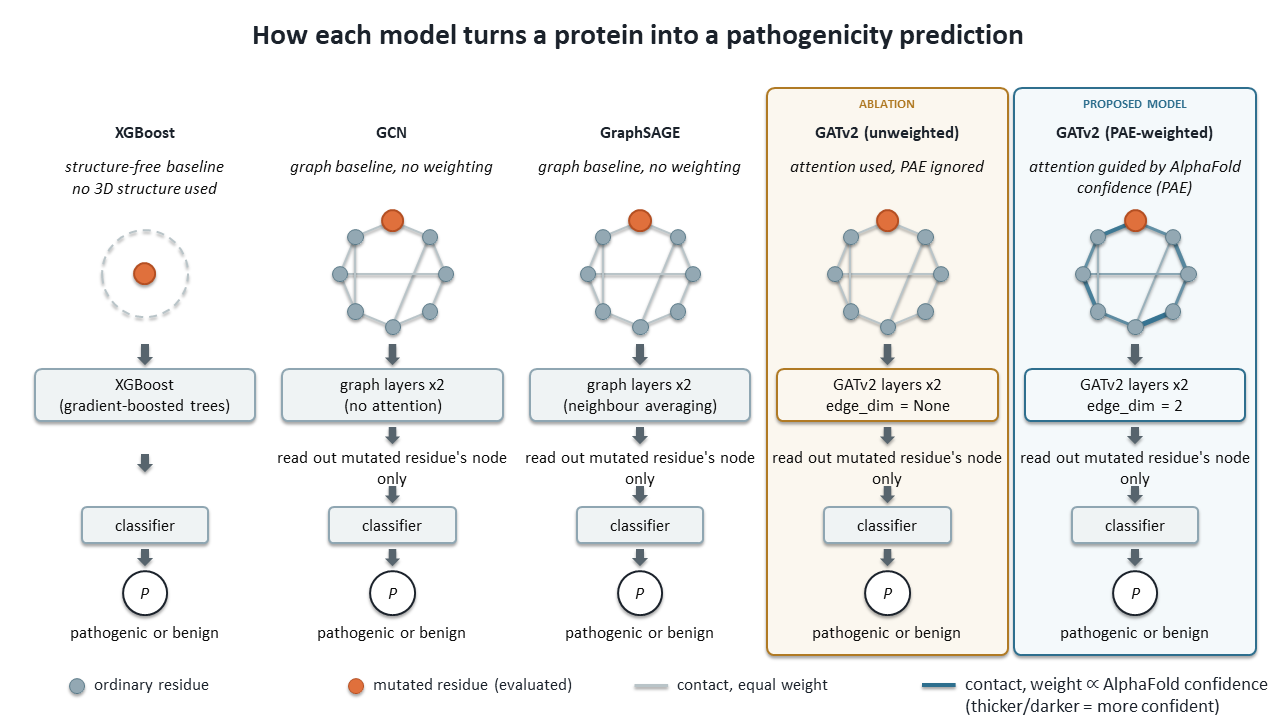
\includegraphics[width=0.92\textwidth]{figures/architecture_comparison.png}
\caption{How each of the five models turns one protein into a single pathogenicity prediction. All five read out only the mutated residue's own representation before classifying it; what differs between them is what information is allowed to reach that representation. The two boxed panels are this paper's central comparison: identical architectures except for whether the edges carry AlphaFold's confidence signal.}
\label{fig:architecture}
\end{figure*}

\textbf{Input and output, model by model.} Every model produces the same kind of output: a single number between 0 and 1, its estimate of how likely this specific variant is to be pathogenic. What differs between them is the input each one is allowed to see.
\begin{itemize}
\item \textbf{XGBoost} sees only the mutated residue's own flat feature vector, 1{,}320 numbers made up of its ESM-2 embedding, wild-type one-hot, and alternate one-hot. There is no graph and no information from any neighbouring residue.
\item \textbf{GCN and GraphSAGE} see the whole protein graph: every residue as a node carrying the 1{,}321-number feature vector described above, and every contact within 8\r{A} as an edge. Neither model reads any number attached to an edge, only whether it exists.
\item \textbf{GATv2 (unweighted)} also sees the full graph, but, like GCN and GraphSAGE, ignores any number carried on an edge. Its attention weights are learned purely from node features.
\item \textbf{GATv2 (PAE-weighted)} sees the same graph, except each edge additionally carries the two numbers described above, distance and PAE weight, which the attention mechanism can use directly.
\item \textbf{AlphaMissense} is not given any input by this study at all: its own precomputed, published score is looked up for each test variant.
\end{itemize}

\subsection{Training setup}
\label{sec:training}

All GNNs were trained with binary cross-entropy loss, weighted by the training split's class ratio (pos\_weight $\approx 1.47$) to counteract the $\sim$60/40 benign/pathogenic imbalance. Protein sizes range up to 2{,}699 residues, so a fixed number of \textit{graphs} per batch is unsafe on limited GPU memory: a measured worst case of 16 large proteins in one batch peaked at 7.26\,GB against a 6.44\,GB budget. A custom sampler instead caps the total \textit{residue count} per batch at 20{,}000, bounding peak memory regardless of shuffle order. Training ran for up to 60 epochs with early stopping after 10 epochs of no validation-AUPRC improvement, restoring the best checkpoint. A short, six-configuration hyperparameter search, with a 5-epoch budget each since validation AUPRC was observed to peak within the first few epochs, selected a winning configuration: hidden dimension 64, dropout 0.4, learning rate $3\times10^{-4}$, weight decay $10^{-4}$. That configuration was then applied to retrain both the PAE-weighted model and its unweighted ablation to full convergence, keeping the comparison fair. To support independent replication, the protein-level split (seed 42), the winning hyperparameter configuration, and every trained checkpoint referenced in this paper are retained and available on request.

\subsection{Testing PAE-weighting three independent ways}
\label{sec:threeways}

A preliminary diagnostic (Section~\ref{sec:saturation}) showed the baseline PAE transform compresses most edge weights into a narrow band. To check whether this was a property of the specific formula or of the underlying data, two further, architecturally distinct encodings of the same PAE information were tested:

\textbf{(a) Per-protein min-max normalization}: rather than a fixed global curve, each protein's own contact-edge PAE values are rescaled relative to that protein's own range, so its most confident edge always maps to weight 1 and its least confident edge to weight 0, guaranteeing the full $[0,1]$ range is used for every protein individually.

\textbf{(b) Directional (non-symmetrized) edge features}: rather than collapsing $\mathrm{PAE}[i][j]$ and $\mathrm{PAE}[j][i]$ into one averaged number, both directions are kept as two separate edge features ($\mathrm{edge\_dim}=3$: distance, forward-direction weight, reverse-direction weight), recovering information the baseline transform discards before any formula is even applied.

\section{Performance Evaluation}
\label{sec:results}

\subsection{Evaluation metrics}
\label{sec:metrics}

\textbf{Area Under the Precision-Recall Curve (AUPRC)} is the primary metric throughout, chosen over raw accuracy because the $\sim$60/40 class split makes accuracy a poor discriminator: a model predicting the majority class alone can score deceptively well. AUROC, Accuracy, Precision, Recall, and F1 (at a 0.5 probability threshold) are reported as secondary metrics, following the project's evaluation plan.

\textbf{Statistical significance} between any two models' predictions on the same test variants is assessed with three complementary paired tests, since predictions from different models on identical variants are correlated and a plain confidence-interval comparison would understate the evidence. McNemar's test is threshold-dependent, comparing correct and incorrect calls directly. A paired bootstrap on the AUPRC difference uses 2{,}000 resamples and is threshold-free. DeLong's test is the standard paired test for two correlated AUROC curves \cite{delong1988auc}. A difference is reported as significant if either the bootstrap or DeLong test yields $p<0.05$, since these rank-based tests are more statistically powerful than the threshold-dependent McNemar's test.

\textbf{PAE Value Quantification} is the percentage change in test AUPRC between the PAE-weighted model and its unweighted ablation, the project's specific pre-registered success criterion for its central hypothesis.

\subsection{Why the baseline PAE transform might not carry much signal}
\label{sec:saturation}

Before training anything, we checked directly whether the assumption underlying PAE-weighting actually holds: that PAE varies enough across a protein's edges to give an attention mechanism something to discriminate on. Sampling 300 proteins (1{,}678{,}270 edges), the 50th, 75th, 95th, and 99th percentiles of $w_{ij}$ were \textit{all exactly 0.5} (mean 0.399, std 0.121). This happens because AlphaFold rarely reports a PAE below $\sim$1\r{A} for two \textit{different} residues, which caps the transform's practical ceiling at $1/(1+1)=0.5$ rather than its analytic maximum of 1.0. It also happens because residue pairs close enough to pass the 8\r{A} contact cutoff are disproportionately the pairs AlphaFold is already confident about. At least half of all sampled edges are therefore numerically indistinguishable from one another.

\subsection{Main comparison: does PAE-weighting help?}

\begin{table}[!ht]
\centering
\caption{Training- and test-set results, all models (train n=34{,}732; test n=6{,}771).}
\label{tab:main-results}
\resizebox{\linewidth}{!}{%
\begin{tabular}{@{}lcccccc@{}}
\toprule
 & \multicolumn{3}{c}{Train} & \multicolumn{3}{c}{Test} \\
\cmidrule(lr){2-4} \cmidrule(lr){5-7}
Model & AUPRC & AUROC & F1 & AUPRC & AUROC & F1 \\
\midrule
GraphSAGE (baseline) & 0.9546 & 0.9677 & 0.8843 & \textbf{0.9148} & 0.9393 & 0.8405 \\
XGBoost (no structure) & 0.9856 & 0.9892 & 0.9410 & 0.9125 & 0.9354 & 0.8305 \\
GATv2 (PAE-w., original) & 0.9840 & 0.9882 & 0.9406 & 0.9112 & 0.9373 & 0.8407 \\
GATv2 (unweighted, original) & 0.9670 & 0.9758 & 0.8942 & 0.9112 & 0.9358 & 0.8273 \\
GATv2 (unweighted, tuned) & 0.9490 & 0.9632 & 0.8836 & 0.9097 & 0.9355 & 0.8354 \\
GATv2 (PAE-w., tuned) & 0.9612 & 0.9715 & 0.9002 & 0.9069 & 0.9339 & 0.8313 \\
GCN (baseline) & 0.9485 & 0.9635 & 0.8819 & 0.8938 & 0.9265 & 0.8104 \\
\bottomrule
\end{tabular}}
\end{table}

Table~\ref{tab:main-results} shows all seven models trained in this study, evaluated on both the training set and the complete test set. AlphaMissense is deliberately left out of this particular table: its publicly released scores cover only 6{,}647 of these 6{,}771 test variants (98.2\%), so adding it here would either misrepresent its coverage or force every other model down to a smaller, less complete test set for the sake of one row. It is instead benchmarked separately, on the matched subset where the comparison is exact, in Section~\ref{sec:ammbench}. Every model scores noticeably higher on the training set than the test set, most visibly XGBoost (0.9856 vs.\ 0.9125 AUPRC) and the original, untuned PAE-weighted GATv2 (0.9840 vs.\ 0.9112); this is the expected signature of these models fitting the training data more closely than they generalise, not a sign anything is wrong with the split or the evaluation. GraphSAGE, the architecturally simplest graph model, with no attention and no edge weighting at all, was nonetheless the best-performing model built in this project on the test set. The PAE-weighted and unweighted GATv2 models are, at every stage, within 0.003 test AUPRC of one another.

\begin{figure}[!ht]
\centering
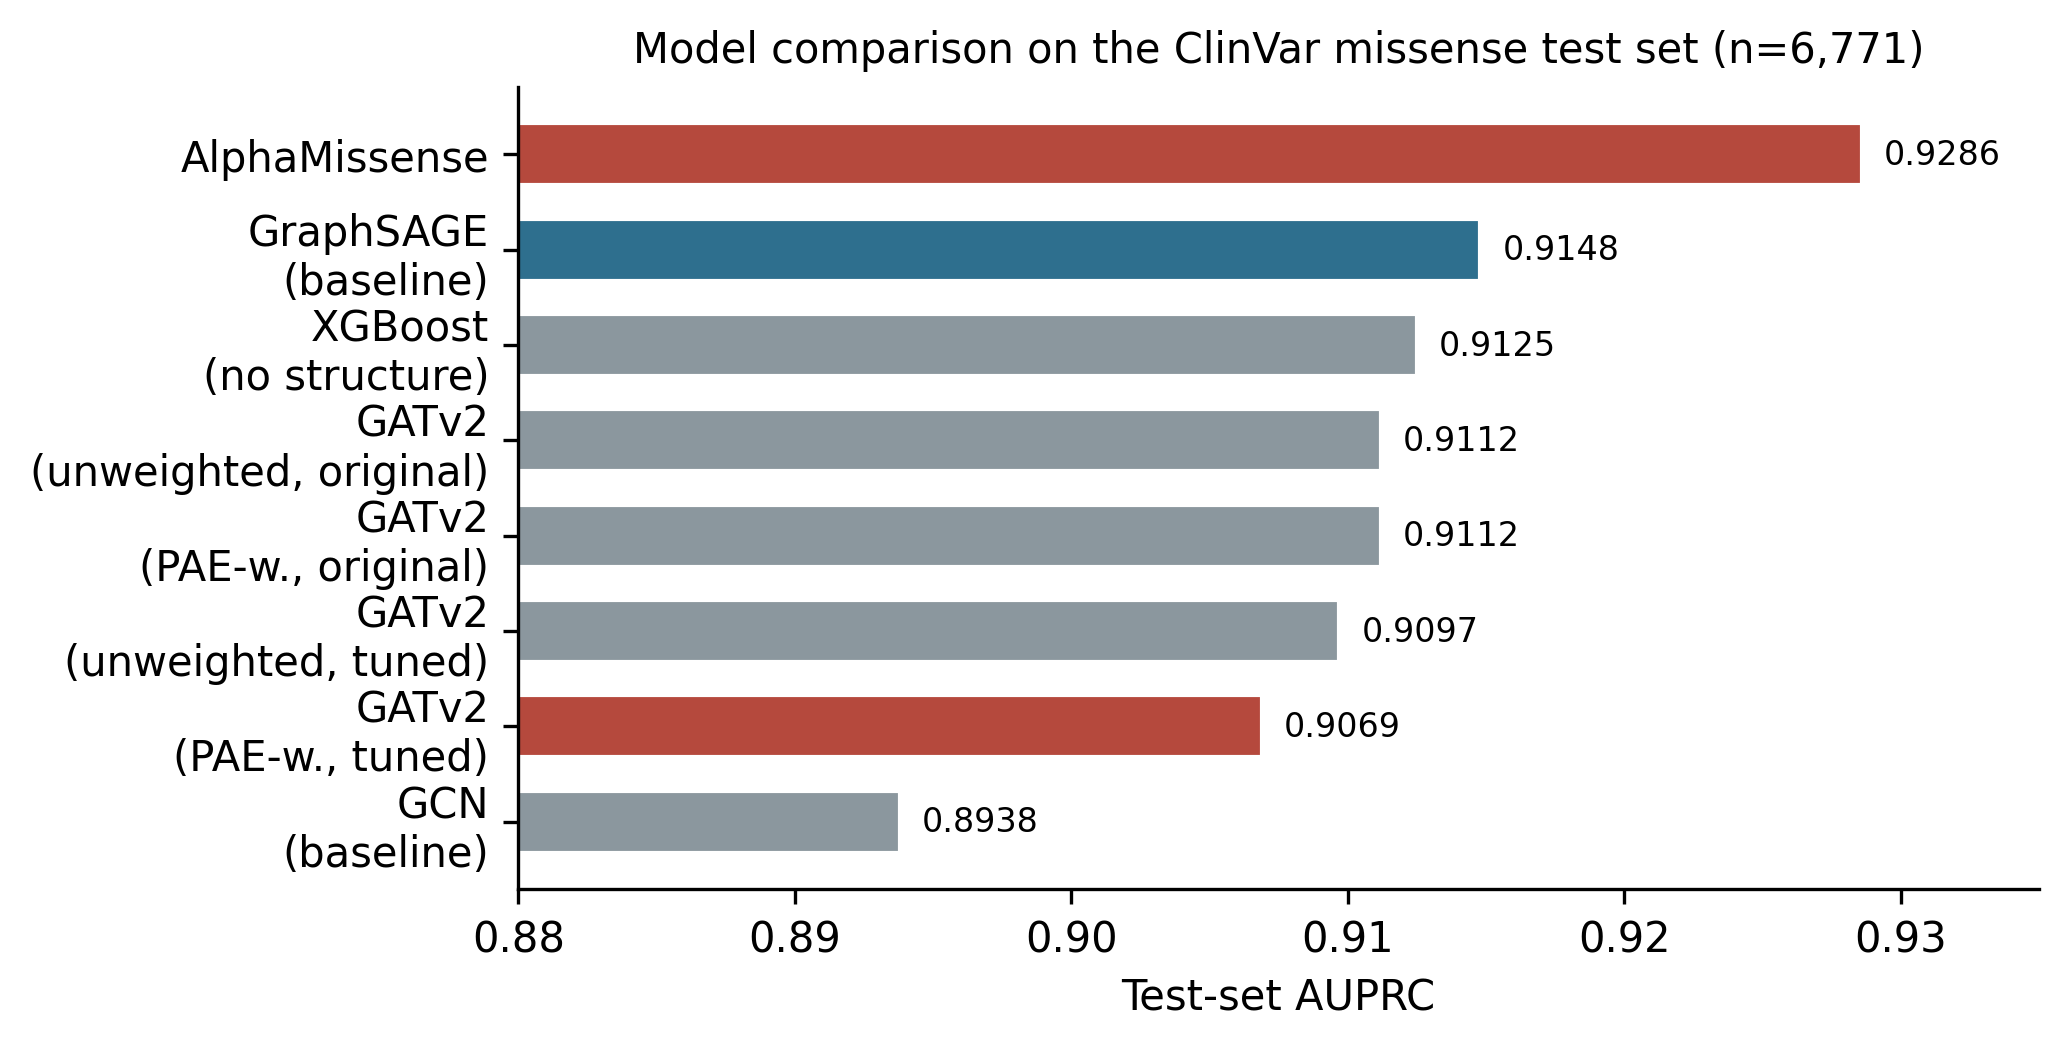
\includegraphics[width=0.48\textwidth]{figures/fig1_model_comparison.png}
\caption{Test AUPRC across all models. The proposed PAE-weighted model (highlighted) does not separate from its unweighted ablation, and both trail GraphSAGE, XGBoost, and AlphaMissense.}
\label{fig:comparison}
\end{figure}

Table~\ref{tab:significance} reports paired significance tests. The core comparison, PAE-weighted versus unweighted, both tuned identically, is \textit{not} statistically significant (bootstrap $p=0.073$, DeLong $p=0.067$), despite AUPRC being nominally lower for the PAE-weighted model. Both variants of GATv2 are, however, significantly behind GraphSAGE. Tuning itself also significantly \textit{hurt} the PAE-weighted model relative to its own untuned version ($p=0.0098$), a sign that the six-configuration search, budgeted for a 5-epoch early read rather than full convergence, did not reliably transfer to full training.

\begin{table}[!ht]
\centering
\caption{Paired significance tests (tuned models unless noted). Bold = significant at $\alpha$=0.05.}
\label{tab:significance}
\small
\begin{tabular}{@{}lcc@{}}
\toprule
Comparison & Bootstrap $p$ & DeLong $p$ \\
\midrule
PAE-w.\ vs.\ unweighted & 0.073 & 0.067 \\
PAE-w.\ vs.\ GraphSAGE & \textbf{0.000} & \textbf{2.7$\times10^{-6}$} \\
PAE-w.\ vs.\ XGBoost & \textbf{0.023} & 0.358 \\
PAE-w.\ (orig.)\ vs.\ PAE-w.\ (tuned) & 0.052 & \textbf{0.0098} \\
\bottomrule
\end{tabular}
\end{table}

A 3-fold cross-validation of the tuned PAE-weighted model, using three different random protein-level splits, gave AUPRC $0.9078 \pm 0.0024$ (range 0.9054-0.9102). That tight spread indicates the model's overall performance level is stable across different held-out proteins, independent of the PAE-weighting question itself.

\textbf{PAE Value Quantification}, this project's pre-registered success metric, tells a consistent story: the PAE-weighted model's AUPRC was \textbf{$-0.31\%$} relative to its unweighted ablation at the tuned stage (0.9069 vs.\ 0.9097), and $+0.004\%$ at the untuned stage, which is statistically indistinguishable from zero ($p=0.94$). Neither reaches the "significant increase" the project's own success criterion required to validate the core hypothesis.

\subsection{Does structure matter at all?}

XGBoost, using no graph and no structural information whatsoever, scored 0.9125 AUPRC, second-best of all seven models and ahead of every GATv2 variant and GCN. A direct head-to-head test between GraphSAGE (the best structural model) and XGBoost (the best non-structural model) gave a small AUPRC gap (+0.0024) that was significant by DeLong's test ($p=0.0085$) but not by the paired bootstrap ($p=0.264$). That disagreement between two legitimate tests suggests any benefit from structure here is real but marginal, nowhere near as robust as the gaps against AlphaMissense reported below.

This marginal benefit is specific to \textit{spatial} structure, not graphs in general. Ghadie et al.\ report the opposite pattern for a graph built on a very different substrate: a disease-specific knowledge graph connecting eleven biomedical entity types raised balanced accuracy from 62\% (language-model embeddings alone) to 85.6\% once a 2-layer GCN was added over it \cite{ghadie2025diseasespecific}. Read together with our own result, this suggests that the specific \textit{kind} of graph substrate matters more than whether a graph is used at all: a 3D spatial-contact graph adds little here, while a curated relational graph over biomedical knowledge added a great deal there.

\subsection{Robustness check: three independent PAE encodings}

To rule out the specific transform formula as the reason PAE-weighting showed no benefit, two further encodings were tested (Section~\ref{sec:threeways}), each trained to the same tuned and untuned configurations.

\textbf{Per-protein min-max normalization.} Before training, a mechanistic diagnostic motivated this specific alternative: any \textit{monotonic} transform of PAE, which both the baseline and min-max transforms are, necessarily preserves which edges tie with one another, since a monotonic function cannot re-order or un-tie values. Table~\ref{tab:minmax-diag} confirms this directly on the same 300-protein sample: the per-protein standard deviation of edge weights is statistically identical between the two transforms, and the fraction of edges tied at each transform's own ceiling value is \textit{exactly} the same. Both configurations were nonetheless trained to full convergence, to confirm this held empirically and not just in theory. At the tuned stage, min-max PAE-weighting (AUPRC 0.9093) was the closest of any encoding tested to its unweighted ablation (bootstrap $p=0.698$, DeLong $p=0.901$). At the untuned/default stage, min-max PAE-weighting (AUPRC 0.9060) was instead \textit{significantly worse} than its unweighted counterpart (bootstrap $p=0.037$). That is the one comparison, across three encodings and two hyperparameter stages each, that reached significance, and it points in the direction of PAE-weighting hurting rather than helping, reinforcing rather than complicating the paper's overall conclusion.

\begin{table}[!ht]
\centering
\caption{Min-max normalization vs.\ baseline transform (300-protein sample).}
\label{tab:minmax-diag}
\small
\resizebox{\linewidth}{!}{%
\begin{tabular}{@{}lcc@{}}
\toprule
 & Baseline $1/(1{+}\mathrm{PAE})$ & Per-protein min-max \\
\midrule
Per-protein std (mean) & 0.1106 & 0.1114 \\
Per-protein std (median) & 0.1156 & 0.1060 \\
Edges at own ceiling & 50.5\% & 50.5\% \\
\bottomrule
\end{tabular}}
\end{table}

\begin{figure}[!ht]
\centering
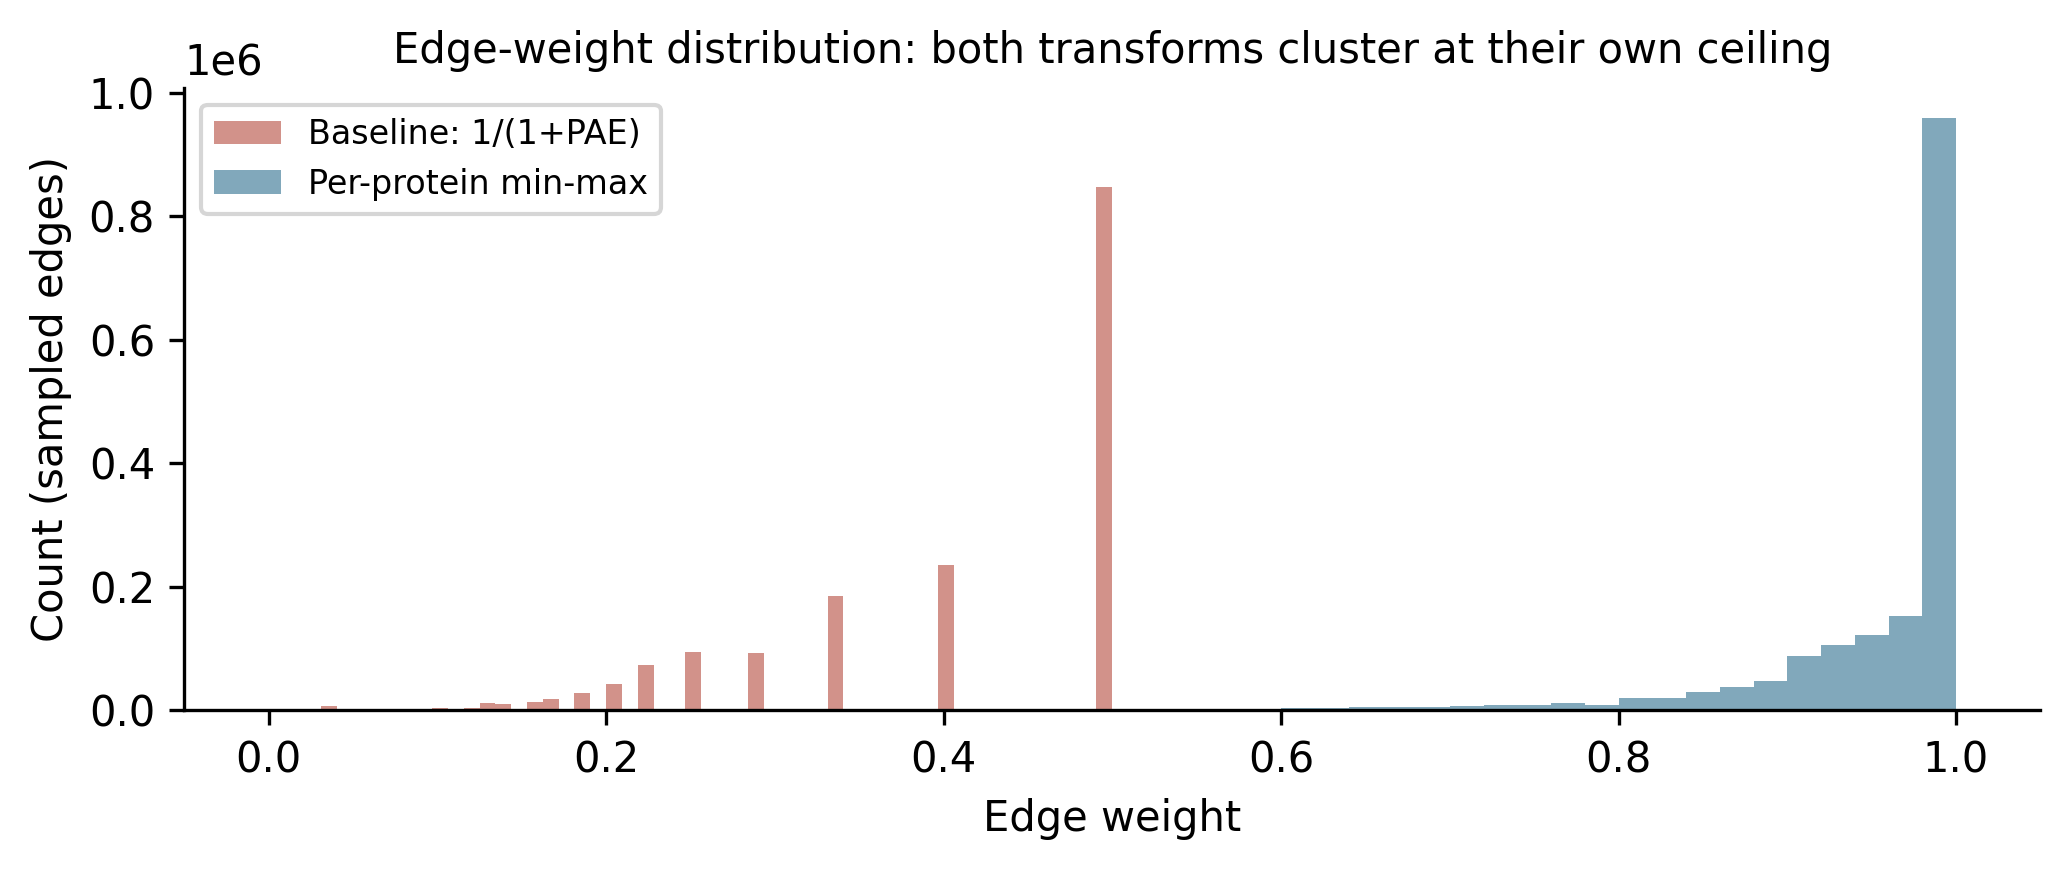
\includegraphics[width=0.48\textwidth]{figures/fig3_saturation.png}
\caption{Both transforms compress most sampled edges toward their own ceiling ($0.5$ for the baseline, $1.0$ for min-max), confirming the effect is a property of the underlying PAE data, not the formula.}
\label{fig:saturation}
\end{figure}

\textbf{Directional (non-symmetrized) edge features} were trained to full convergence for a different reason: this is not a reformulation but a genuine recovery of previously discarded information. Table~\ref{tab:tie-breaking} quantifies how much of edges tied under the symmetrized baseline transform, 32.8\% actually have $\mathrm{PAE}[i][j]\neq\mathrm{PAE}[j][i]$ in AlphaFold's raw output, information the averaging step erases, while 67.2\% are tied even with full directional information restored. That is a genuine, partial, but not complete, recovery of discarded signal.

\begin{table}[!ht]
\centering
\caption{Tie-breaking from recovering directional PAE (300-protein sample, 1{,}678{,}270 edges).}
\label{tab:tie-breaking}
\small
\begin{tabular}{@{}lc@{}}
\toprule
Quantity & Value \\
\midrule
Edges tied under symmetrized transform & 100\% \\
\quad of those, distinguishable via direction & 32.8\% \\
\quad of those, genuinely tied (both directions equal) & 67.2\% \\
\bottomrule
\end{tabular}
\end{table}

\textbf{All three encodings, compared.} Table~\ref{tab:all-encodings} places all three tuned models side by side against the unweighted ablation. None reaches significance at the tuned stage, which is the fully-converged, hyperparameter-matched configuration used for the paper's main comparison throughout (bootstrap $p=0.073$-$0.698$, DeLong $p=0.067$-$0.901$). Min-max is numerically closest to the unweighted ablation; the baseline transform is numerically furthest; directional sits between the two. All three point the same direction: no evidence that PAE-weighting helps, regardless of how the same underlying AlphaFold confidence signal is encoded.

\begin{table}[!ht]
\centering
\caption{All three PAE encodings vs.\ unweighted ablation (tuned models).}
\label{tab:all-encodings}
\small
\resizebox{\linewidth}{!}{%
\begin{tabular}{@{}lccc@{}}
\toprule
Encoding & AUPRC & Bootstrap $p$ & DeLong $p$ \\
\midrule
Baseline (symmetrized, $1/(1{+}\mathrm{PAE})$) & 0.9069 & 0.073 & 0.067 \\
Per-protein min-max & 0.9093 & 0.698 & 0.901 \\
Directional ($\mathrm{edge\_dim}{=}3$) & 0.9074 & 0.092 & 0.140 \\
\bottomrule
\end{tabular}}
\end{table}

Across six tested comparisons, three encodings times two hyperparameter stages each, exactly one reached significance: untuned min-max, and in the direction of PAE-weighting hurting, not helping. Three independent encodings of the same underlying AlphaFold confidence signal, a reformulation, a per-protein rescaling, and a genuine information recovery, converge on the same conclusion, ruling out "wrong formula" as an explanation for the null result.

\subsection{Benchmarking against AlphaMissense (RQ1, RQ3)}
\label{sec:ammbench}

On the 98.2\% of test variants with a published AlphaMissense score (6{,}647 of 6{,}771), AlphaMissense scored 0.9286 AUPRC against GraphSAGE's 0.9159, the baseline PAE-weighted model's 0.9073, the min-max PAE-weighted model's 0.9101, and the directional PAE-weighted model's 0.9081 (Fig.~\ref{fig:alphamissense}). The matched-subset pathogenic rate of 39.9\% closely tracks the full test set's 40.2\%, so there is no meaningful selection bias from the match. Every pairwise comparison against AlphaMissense was significant at this paper's $p<0.05$ threshold, unlike most of the internal PAE-weighting-versus-unweighted comparisons above. The gap was strongest for all three PAE-weighted encodings, each reaching $p<0.001$ on both the bootstrap and DeLong tests; GraphSAGE's own gap against AlphaMissense, while still significant, was comparatively less extreme (bootstrap $p=0.001$, DeLong $p=0.013$). AlphaMissense's advantage is real, large, and consistent regardless of edge encoding, reflecting its much larger training scale, roughly 19{,}000 proteins with population-frequency labels, rather than any architectural choice tested in this paper.

\begin{figure}[!ht]
\centering
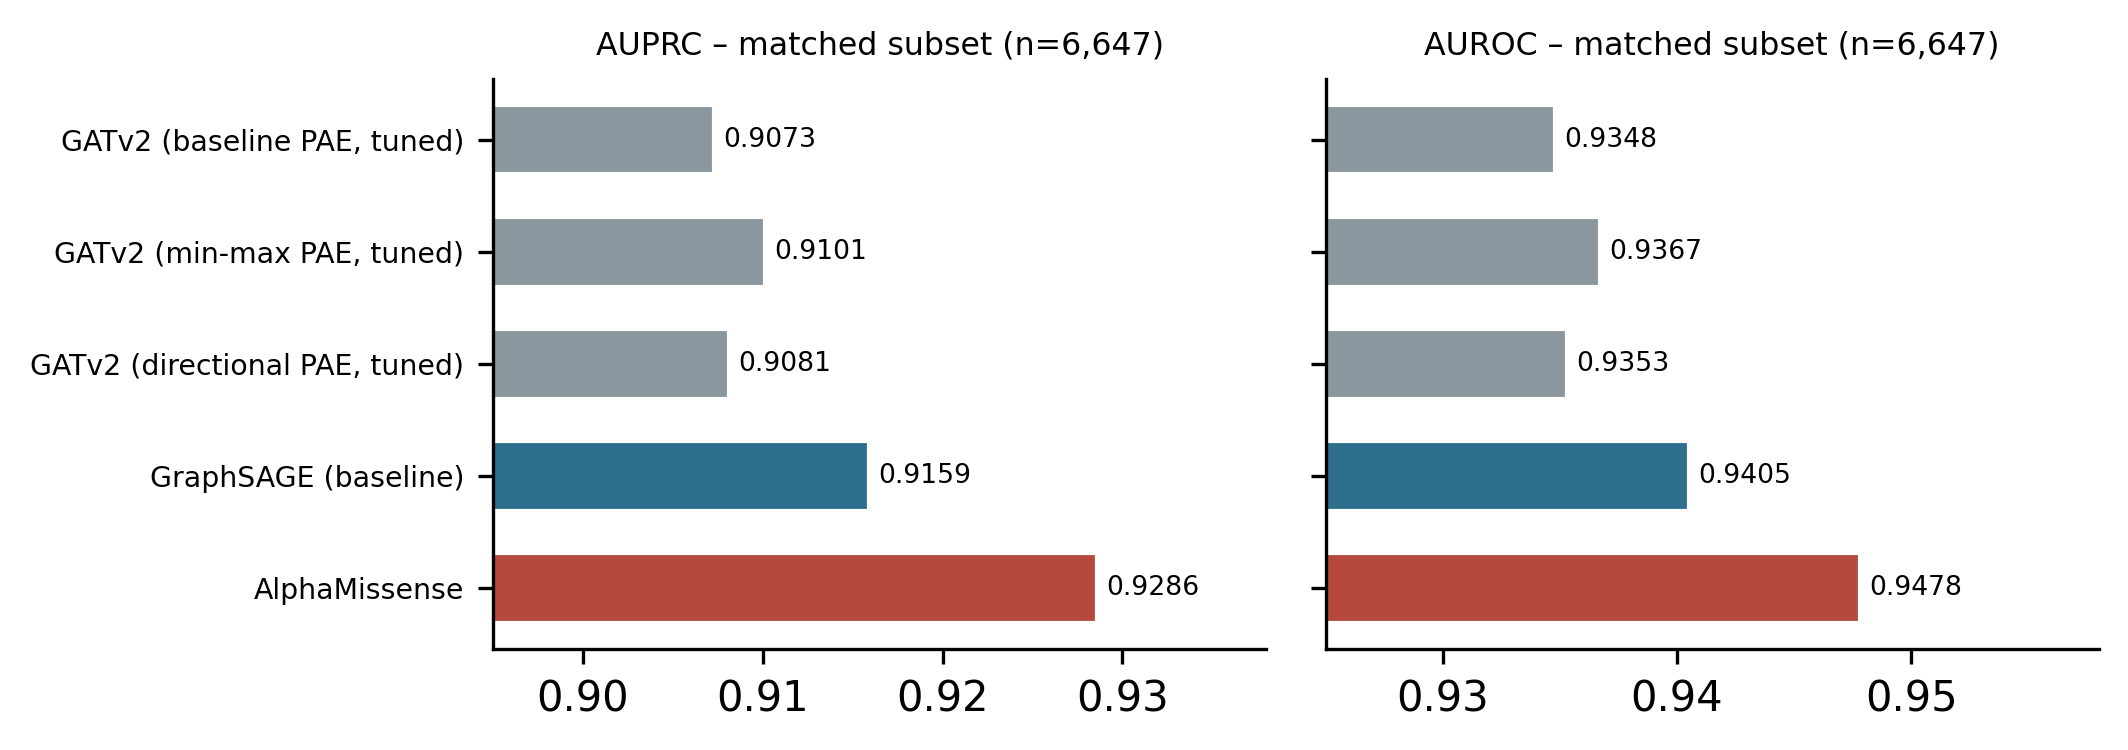
\includegraphics[width=0.48\textwidth]{figures/fig2_alphamissense_comparison.png}
\caption{AUPRC and AUROC on the matched AlphaMissense test subset (n=6{,}647), for all three PAE encodings, GraphSAGE, and AlphaMissense.}
\label{fig:alphamissense}
\end{figure}

\subsection{Exploratory application to real Variants of Uncertain Significance}
\label{sec:vus}

Every result reported above uses ClinVar variants that already carry a confirmed Pathogenic or Benign label, which is necessary for evaluation but sidesteps the real-world problem that motivated this paper: the roughly 98\% of missense variants with no confirmed classification at all, ClinVar's Variants of Uncertain Significance (VUS). As an exploratory extension, the tuned PAE-weighted model was applied to real ClinVar VUS restricted to the 6{,}597 proteins already covered by this project's structural graphs, so no new AlphaFold, ESM-2, or UniProt data was required. After the same quality filters used for the main dataset (Section~\ref{sec:data}), this yielded \textbf{207,266 VUS across 4,053 proteins}. \textbf{28.5\%} of these scored above the model's 0.5 decision threshold (mean probability 0.312, median 0.137). This is reported descriptively, not as a validation: VUS have no ground-truth label by definition, so there is nothing to check these predictions against, and the result should not be read as evidence the model performs well on this population, only as a demonstration of what applying it looks like. The full per-variant output, together with the exact ClinVar snapshot and model checkpoint used, is preserved for inspection in \textit{vus\_prediction.py} and its saved outputs.

\section{Conclusion}
\label{sec:conclusion}

\subsection{Answering the research questions}

\textbf{RQ1: Not supported.} The PAE-and-ESM-2 GNN did not significantly outperform existing methods; AlphaMissense remained significantly ahead throughout.

\textbf{RQ2: Not supported, and now mechanistically understood.} PAE-weighted edges added no significant value over an unweighted ablation at the tuned stage. This was confirmed across three independent, fully-trained encodings of the same underlying signal, including one that recovered directional information the baseline transform discards. The single significant result across all six tested configurations, untuned min-max, pointed the same direction, toward PAE-weighting hurting rather than helping. The saturation diagnostic in Section~\ref{sec:saturation} gives a concrete, falsifiable reason why: AlphaFold rarely reports sub-1\r{A} confidence for distinct residue pairs, and residue pairs passing a standard contact cutoff are disproportionately the ones AlphaFold is already confident about, leaving little variation for an attention mechanism to exploit.

\textbf{RQ3: Not supported.} A model trained only on high-confidence clinical labels did not outperform AlphaMissense, which benefits from population-scale training data no ClinVar-only model of this size can match.

\subsection{Assumptions}

This study rests on several explicit assumptions, made necessary by the scale of the dataset and the practical limits of GPU-constrained training. They are stated here directly rather than left implicit, since some of them turned out not to hold and that is itself part of the result.
\begin{itemize}
\item AlphaFold2's predicted structure is assumed to be an adequate stand-in for a variant's true 3D conformation. Only a minority of the proteins in this dataset have an experimentally solved structure available to check that assumption against directly.
\item The standard 8\r{A} alpha-carbon cutoff is assumed to capture the physical contacts that matter for a variant's local environment. A looser or tighter cutoff was not explored, and a different cutoff could in principle change which residues ever have the chance to influence a prediction.
\item Symmetrizing PAE into one averaged confidence value per edge, the baseline transform, is assumed to be a reasonable simplification of AlphaFold's inherently directional confidence output. This assumption is not merely asserted: Section~\ref{sec:threeways}'s directional encoding tests it directly, and finds the simplification defensible, since most of the information it discards turns out to be redundant (Table~\ref{tab:tie-breaking}).
\item ClinVar's Pathogenic and Benign labels, after filtering to 2-star-or-better review status, are treated as ground truth. Expert curators do occasionally revise a classification as new evidence emerges, so a small fraction of labels may not reflect current clinical consensus.
\item The six-configuration hyperparameter search was assumed to transfer from a 5-epoch early read to full 60-epoch training. Table~\ref{tab:significance} shows this assumption did not hold for the PAE-weighted model: tuning on an early signal significantly changed its fully-converged performance, and this is reported as a finding rather than smoothed over.
\item Two rounds of GATv2 message passing were assumed to give the mutated residue's representation enough reach into its structural neighbourhood. Deeper stacks were not tested, partly because GPU memory was already the binding constraint described in Section~\ref{sec:training}.
\end{itemize}

\subsection{Limitations}

The protein-level split, while leakage-safe, is a harder test than a variant-level split and may depress all models similarly. Six of seven models were evaluated on a single train/test split; only the PAE-weighted model received 3-fold cross-validation. GPU memory constraints required node-budget batching rather than a fixed batch size. The 0.5 classification threshold was not calibrated per model. The two additional PAE encodings tested are not exhaustive: they rule out monotonic reformulation and directional-information loss specifically, not every conceivable encoding. The exploratory VUS application (Section~\ref{sec:vus}) is descriptive only; because VUS have no ground-truth label, its 28.5\% predicted-pathogenic rate cannot be validated and should not be read as an accuracy estimate. All seven models score noticeably higher on the training set than the test set (Table~\ref{tab:main-results}), a normal sign of overfitting given the dataset's size. This does not change the paper's central conclusion, since RQ2's PAE-weighted-versus-unweighted comparison uses the same architecture and training procedure on both sides, which overfit by a similar amount, keeping that comparison fair. Overfitting may still be part of why this project's models fall short of AlphaMissense in Section~\ref{sec:ammbench}, though AlphaMissense's much larger training scale, roughly 19{,}000 proteins versus 6{,}597 here, is a more likely explanation for most of that gap.

\subsection{Future work}

Beyond the specific null result, the saturation diagnostic introduced in Section~\ref{sec:saturation}, checking whether a candidate edge-weighting signal actually has enough spread across the edges a fixed contact cutoff selects before spending GPU time training a full model on it, is intended as a reusable first check for future work considering PAE, or any similarly bounded confidence score, as a graph edge weight. Three directions, distinct from what has been ruled out here, remain untested. First, using PAE to determine graph \textit{topology}, which contacts exist at all, rather than only edge \textit{weight}, how much an existing contact is trusted, is a qualitatively different lever. Second, combining PAE with co-evolution, the signal gMVP already showed to be useful, tests a joint hypothesis that neither signal alone has been shown to satisfy here. Third, using PAE to reweight training loss per-variant, rather than as a model input feature, shifts it from an architectural signal to a training-time one. Fourth, the 207,266 VUS predictions produced in Section~\ref{sec:vus} could be tracked prospectively: as ClinVar reclassifies a portion of today's VUS into confirmed Pathogenic or Benign calls over time, checking whether this model's predictions agreed with the eventual reclassification would turn today's purely descriptive exploratory pass into an actual, if slow, validation. Given the consistency of the null result across three independent encodings in this study, we recommend these be treated as open questions for future work rather than incremental variations on the same idea.

\section{Generative AI Disclosure}

Generative AI was used solely for limited linguistic assistance to improve the manuscript's clarity, readability, and grammar. It was also used to generate the architectural diagrams in this paper based on author-provided specifications.

\bibliographystyle{IEEEtran}
\bibliography{references}

\end{document}
